\documentclass[12pt]{article}
\usepackage[T2A]{fontenc}
\usepackage[utf8]{inputenc}
\usepackage{multirow}
\usepackage{caption}
\usepackage{subcaption}
\usepackage{amsmath}
\usepackage{changepage}
\usepackage{graphicx}
\usepackage{float}
\usepackage[english,russian]{babel}
\usepackage{amsmath, amsfonts, amssymb, amsthm, mathtools}
\usepackage{xcolor}
\usepackage{array}
\usepackage{hyperref}
\usepackage{icomma}
\usepackage{mathtext} 
\usepackage[top = 1.5cm, left = 1.5 cm, right = 1.5 cm, bottom = 3 cm]{geometry}
\graphicspath{ {./images/} }
 
\date{\today}
  
\begin{document}
\begin{titlepage}
	\begin{center}
		{\large МОСКОВСКИЙ ФИЗИКО-ТЕХНИЧЕСКИЙ ИНСТИТУТ (НАЦИОНАЛЬНЫЙ ИССЛЕДОВАТЕЛЬСКИЙ УНИВЕРСИТЕТ)}
	\end{center}
	\begin{center}
		{\large Физтех-школа физики и исследований им. Ландау}
	\end{center}

	\vspace{3cm}
	{\huge
		\begin{center}
			\textbf{Исследование самовозбуждающихся режимов работы схемы Чуа.}
		\end{center}
	}
	\vspace{2cm}
	\begin{flushright}
		{\LARGE Автор:\\ Шахматов Андрей Юрьевич \\
			\vspace{0.2cm}
			Б02-304}
	\end{flushright}
	\vspace{7 cm}
	\begin{center}
		Долгопрудный 2024
	\end{center}
	\thispagestyle{empty}
\end{titlepage}

% \maketitle

\begin{abstract}
	Надо написать.
\end{abstract}

% \tableofcontents

\section*{Введение}
В современном мире проблема обеспечения безопасности информации становится все более актуальной.
Одним из перспективных решений данной задачи является использование хаотических сигналов в качестве несущей волны.
Такой подход значительно повышает уровень защиты данных,
так как злоумышленник сталкивается с практически неразрешимой задачей расшифровки хаотического сигнала.

Для генерации хаотических сигналов широко применяется схема Чуа, включающая два конденсатора,
индуктивность, сопротивление и нелинейный элемент --- диод Чуа.
Простота конструкции делает эту схему привлекательной для различных отраслей промышленности.
Однако, несмотря на наличие теоретической модели, описывающей поведение схемы Чуа,
её практическое применение сталкивается с рядом сложностей, такими как высокая чувствительность контура и
ограниченная область хаотического поведения.

Целью данной работы является детальное исследование хаотических режимов работы схемы Чуа,
а также устойчивых нехаотических режимов, сосуществующих с хаотическими.

\section*{Теоретическая часть}
\subsection*{Хаотические системы}
Предметом изучения теории хаоса являются ситемы, описываемые дифференциальными уравнениями вида $$\ddot{x} = v(x,t)$$
Стоит отметить, что левая часть должна быть нелинейной (линейные системы никогда не являются хаотическими). Давайте поймем, какую систему стоит считать хаотической:
\begin{enumerate}
	\item Она обладает свойством сильной зависимости от начальных условий. Кванторно это можно записать так: $\forall \varepsilon > 0 \exists \delta > 0: \forall x,y :  \rho(x,y) < \varepsilon \Rightarrow \rho(g^{\tau}(x),g^{\tau}(y)) > \delta$.
			Геометрически это можно интерпретировать следующим образом:
			\begin{figure}[H]
				\centering
				\includegraphics[width=0.35\textwidth]{dependance_st_pos.png}
				\caption{Демонстрация сильной зависимости поведения системы от начальных условий}
				\label{fig:demonstrate_dependance}
			\end{figure}
	\item Динамическая система должна обладать свойством топологического смешивания (быть транзитивной): то есть для любых двух множеств нашего фазового пространства системы поток от одного рано или поздно должен пересечься со вторым выбранным множеством.
	\item Периодические орбиты системы должны быть всюду плотными в нашем фазовом портрете.
\end{enumerate}

Важным обьектом в вопросе изучения хаотических систем являются аттракторы: подмножества нашего фазового пространства к которому стремятся все наши решения, т.е:
$g^{\tau}(A) = A \quad\&\quad \forall U_{\varepsilon}(A): g^{\tau}(U_{\varepsilon}(A)) \rightarrow A$

\subsection*{Устройство схемы Чуа}
\begin{figure}[H]
	\centering
	\includegraphics[width=0.4\textwidth]{Base_chua_curcuit.png}
	\hfil
	\includegraphics[width=0.35\textwidth]{chua_VAC.png}
	\caption{Электрическая схема цепи Чуа и вольт-амперная характеристика диода Чуа $N_R$.}
	\label{fig:base_curcuit}
\end{figure}
Классическая схема Чуа состоит из двух конденсаторов, сопротивления, индуктивности и диода Чуа.
Диод Чуа возможно реализовать при помощи использования двух операционных усилителей и шести резисторов (Рис. \ref{fig:OA_Gyrator}).
Также в реальности использование физической индуктивности может приводить к плохим результатам из-за наличия большого внутреннего
сопротивления. По этой причине в нашей работе индуктивность была заменена схемой на основе операционных усилителей --- гиратором (Рис. \ref{fig:OA_Gyrator}).
Эквивалентную индуктивность полученной схемы можно расчитать
\begin{eqnarray}
	L = \frac{R_7 R_9 R_{10} C}{R_8},
	\label{eq:gyrator}
\end{eqnarray}
где $R$ пронумерованы в порядке от врехнего к нижнему на схеме.

\begin{figure}[H]
	\centering
	\includegraphics[width=0.35\textwidth]{OA.jpg}
	\hfil
	\includegraphics[width=0.35\textwidth]{gyrator.jpg}
	\caption{Реализация диода Чуа на основе операционных усилителей и эквивалентная индуктивности схема гиратора.}
	\label{fig:OA_Gyrator}
\end{figure}

Применяя полученные модификации получим исходную вариацию схемы с использованием только операционных усилителей, конденсаторов и сопротивлений (Рис. \ref{fig:final_curcuit}).
\begin{figure}[H]
	\centering
	\includegraphics[width=0.55\textwidth]{chua_curcuit.jpg}
	\caption{Итоговая электрическая схема цепи Чуа, использующаяся в данной работе.}
	\label{fig:final_curcuit}
\end{figure}

Резисторы $R$ и $R_{10}$ являются переменными ползунковыми резисторами.
Точные характеристики элементов приведены в приложении (Таблица \ref{tab:curcuit_chars}).

\subsection*{Математическая модель схемы Чуа}
Обозначив за $U_{C_1}, U_{C_2}, I_{L}$ напряжения на конденсаторах и ток через катушку соответственно можно записать систему уравнений, описывающую цепь Чуа: 
\begin{equation}
	\begin{dcases}
		C_1 \frac{d U_{C_1}}{dt} = \frac{U_{C_2} - U_{C_1}}{R} - g(U_{C_1}), \\
		C_2 \frac{d U_{C_2}}{dt} = \frac{U_{C_1} - U_{C_2}}{R} + I_L, \\ 
		L \frac{d I_L}{dt} = -U_{C_2},
	\end{dcases}
	\label{eq:chua_system}
\end{equation} 
где $R$ --- сопротивление резистора, $L$ --- индуктивность катушки, $C_1, C_2$ --- ёмкости конденсаторов, а $g$ --- функция зависимости тока от напряжения 
на диоде Чуа: 
\[
	g(U_{C_1}) = G_b U_{C_1} + \frac{1}{2} \left( G_a - G_b \right) \left( \vert U_{C_1} + E \vert - \vert U_{C_1} - E \vert \right),
\]
где $G_b, G_a, E$ --- проводимости соответствующих участков и точки излома на рисунке \ref{fig:base_curcuit}.

Введя новые обозначения можно привести систему к новым безразмерным переменным: 
\begin{equation}
	\begin{dcases}
		\frac{dx}{d \tau} = \alpha(y - x - h(x)), \\
		\frac{dy}{d \tau} = x - y + z, \\
		\frac{dz}{d \tau} = -\beta y, \\
	\end{dcases}
	\label{eq:chua_system_}
\end{equation}
где $m_0 = R G_a$, $m_1 = R G_b$, $\alpha = \frac{C_2}{C_1}$, $\beta = \frac{R^2 C_2}{L}$, 
$\tau = \frac{t}{R C_2}$, $x = \frac{U_{C_1}}{E}$, $y = \frac{U_{C_2}}{E}$, $z = \frac{I_L R}{E}$, и функция $h(x)$ равна 
\[
	h(x) = m_1 x + \frac{1}{2}(m_0 - m_1)(\vert x + 1 \vert - \vert x - 1 \vert ).
\]

В реальности, однако, вольт-амперная характеристика диода Чуа несколько отличается (Рис. \ref{fig:VAC}), это 
связано с тем, что операционный усислитель не является идеальным и после некторого напряжения появляются возрастающие участки. 
В таком случае удобно определять положения равновесия графически, нужно провести нагрузочную прямую $I = -\frac{U}{R}$ и рассмотреть 
её точки пересечения с вольт-амперной характеристикой диода.
\begin{figure}[H]
	\centering
	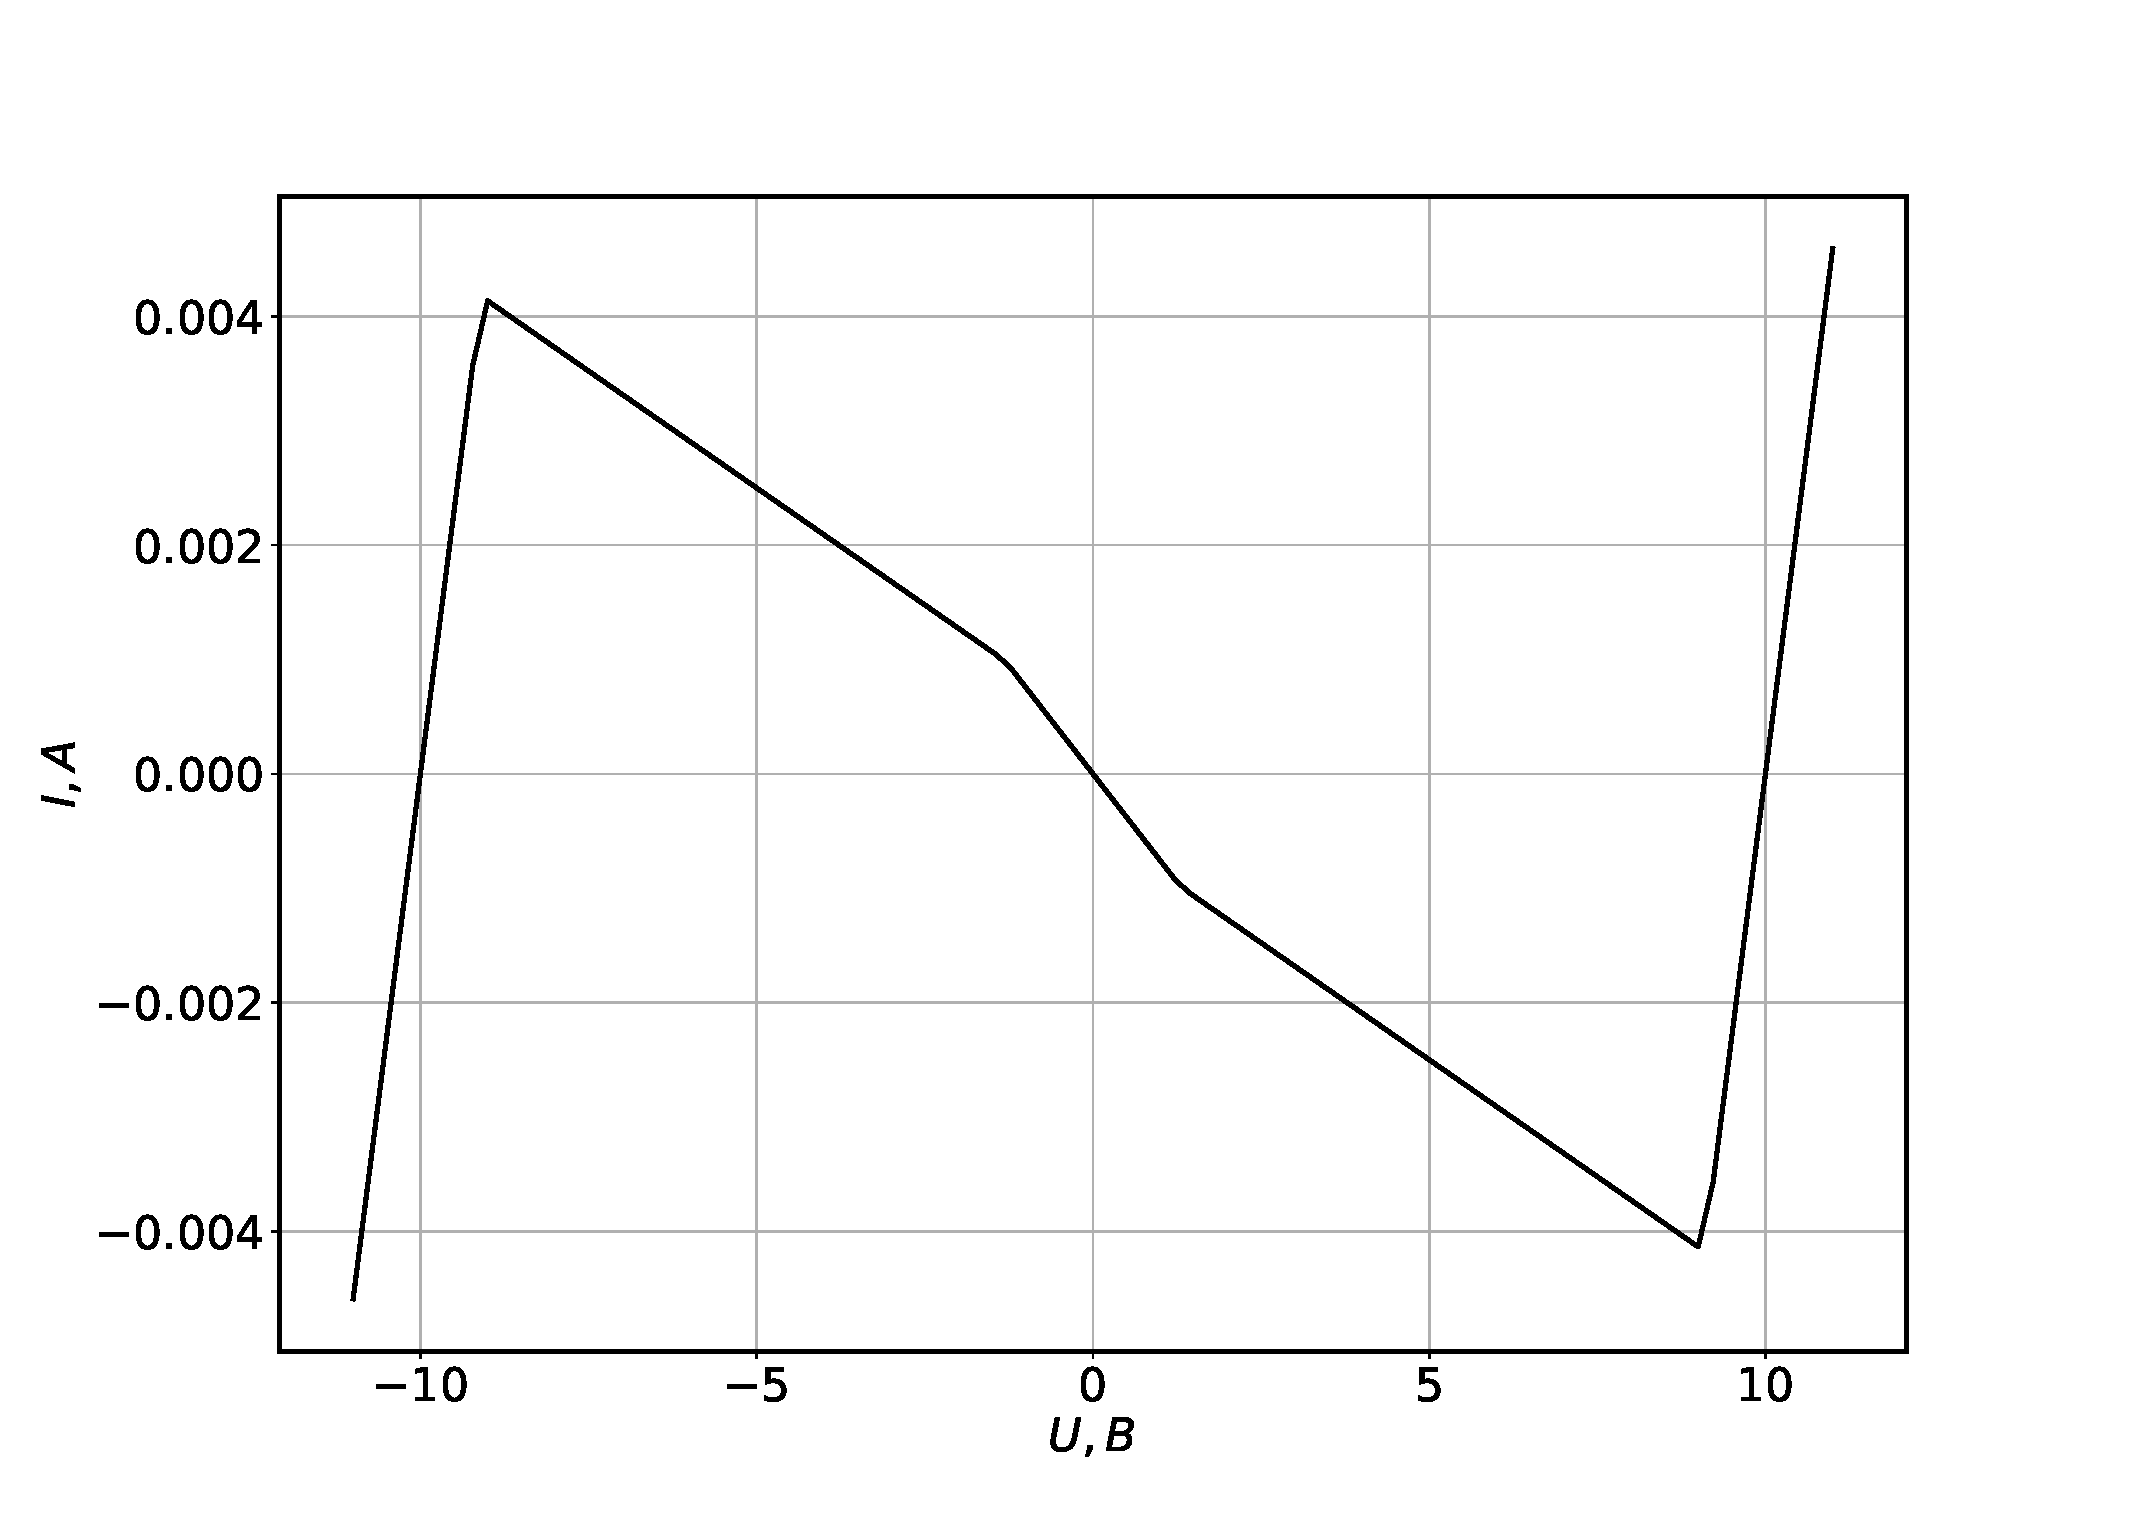
\includegraphics[width=0.6\textwidth]{VAC.eps}
	\caption{Вольт-амперная характеристика диода Чуа, реализованного на операционных усилителях.}
	\label{fig:VAC}
\end{figure}

\section*{Результаты и их анализ}
\subsection*{Численное моделирование бифуркационной диаграммы}
Проведёно численное моделирование схемы Чуа с указанными в приложении параметрами, согласно дифференциальным уравнениям \ref{eq:chua_system}. 
Моделирование проводилось с шагом $\Delta R = 50$ Ом и $\Delta R_L = 150$ Ом. После моделирования получен набор 
изображений фазовых портретов системы при различных её параметрах \ref{fig:simulation}.
\begin{figure}[H]
	\centering
	\includegraphics[width=0.55\textwidth]{sim_ex.png}
	\caption{Пример результата симуляции, полученной при $\Delta R = 110$ Ом и $\Delta R_L = 350$ Ом.}
	\label{fig:simulation}
\end{figure}
На полученной диаграмме можно выделить несколько областей с принципиально различными состояниями. 
По диаграмме определены пограничные кривые между различными состояниями системы и построен график \ref{fig:phase_diag_teor}. 
У системы можно выделить 5 основных состояний: большой предельный цикл, двухпетлевой аттрактор, аттрактор Рёсслера, устойчивый фокус и 
малый предельный цикл. 
Отдельно рассмотрим систему при $R > 2.25$ КОм, в данной области у системы существует три положения равновесия, и нагрузочная 
прямая $-R$ пересекает график диода Чуа (Рис. \ref{fig:VAC}) в точка, которые лежат на крайних правой и левой прямой после второго излома. 
В данной области система может находится только лишь в этих положениях равновесия и на фазовой диаграмме наблюдается точка, изредка 
перескакивающая между положениями равновесия. 
Интересующая нас область хаотического поведения наблюдается при $R < 2.25$ КОм. При больших $R_L$ система переходит 
в большой предельный цикл, который возникает из-за существования второго излома на графке вольт-амперной характеристики диода Чуа. 
При понижении $R_L$ в системе начинает наблюдаться двухпетелевой аттрактор, понижая $R_L$ далее, в системе последовательно 
наблюдается переход сначала в аттрактор Рёсслера, затем в малый предельный цикл, далее в устойчивый фокус и затем снова в предельный цикл. 
При понижении $R$ далее, кривые перехода между состояниями стремяться в одну точку, соответственно при $R_{crit}$ область существования аттракторов 
заканчивается. Это связано с тем, что нагрузочная кривая $R$ совпадает с прямой $G_a$ до первого излома (Рис. \ref{fig:VAC}). 
В такой конфигурации в системе существует бесконечное число положений равновесия и система дрейфует между ними. 
После дальнейшего понижения $R$ в системе существует только одно положение равновесия --- точка $(0, 0, 0)$. В зависимости от его 
устойчивости фазовая диаграмма системы представляет собой либо большой предельный цикл, либо в малый предельный цикл, либо в точку.    


\begin{figure}[H]
	\centering
	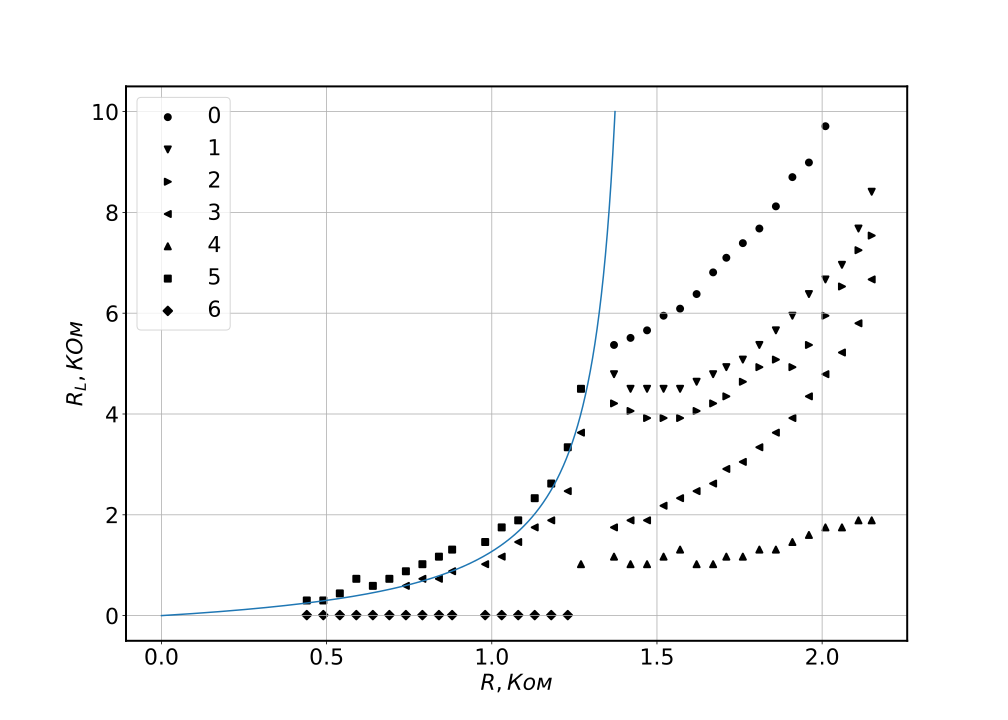
\includegraphics[width=0.75\textwidth]{bif_diag_teor.pdf}
	\caption{Диаграмма состояний системы при различных $R$ и $R_L$. 
	Цифрами обозначены граничные кривые для состояний: 
	0 --- большой предельный цикл и двухпетлевой аттрактор,
	1 --- двухпетлевой аттрактор и аттрактор Рёсслера,\
	2 --- аттрактор Рёсслера и малый предельный цикл,
	3 --- малый предельный цикл и фокус, 
	4 --- фокус и малый предельный цикл, 
	5 --- большой предельный цикл и малый предельный цикл,
	6 --- фокус и малый предельный цикл.}
	\label{fig:phase_diag_teor}
\end{figure}

\subsection*{Теоретическое описание положений равновесия} 
Исследована область при $R < -\frac{1}{G_a}$. При таких параметрах в системе будет одно положение равновесия $(0, 0, 0)$. 
Рассмотрим приведённую систему дифференциальных уравнений \ref{eq:chua_system_}. В таком случае можно исследовать устойчивость положения 
равновесия по линейному приближению. В таком случае система перепишется как: 
\[
	\begin{dcases}
		\frac{dx}{d \tau} = \alpha(y - x - m_0 x), \\
		\frac{dy}{d \tau} = x - y + z, \\
		\frac{dz}{d \tau} = -\beta y. \\
	\end{dcases}
\]
Необходимым и достаточным условием ассимптотической устойчивости является отрицательная действительная часть всех собственных значений 
характеристического многочлена матрицы $f(\lambda)$: 
\[
	f(\lambda) = \lambda^3 + \lambda^2 (1 + \alpha + \alpha m_0) + \lambda (\beta + \alpha m_0) + \alpha \beta + \alpha \beta m_0.
\] 
Согласно критерию Гурвица для выполнения критерия устойчивости необходимо выполнение условия $a_1 a_2 - a_0 a_3 > 0$: 
\[
	(1 + \alpha + \alpha m_0) (\beta + \alpha m_0) - \alpha \beta + \alpha \beta m_0 > 0.
\]
После расскрытия скобок и приведения подобных слагаемых имеем: 
\[
	\beta > -\alpha m_0 - \alpha^2 m_0 - \alpha^2 m_0^2
\]
Вернёмся к исходным обозначениям, $\beta = \frac{C_2 R^2}{L}, m_0 = G_a R$: 
\begin{equation}
	R > -\frac{\alpha + 1}{\alpha G_a + \frac{C_2}{\alpha L G_a}},
	\label{eq:R_crit}
\end{equation}
где $L$ для нашей схемы выражается согласно выражению \ref{eq:gyrator}. В таком случае зависимость 
критического значения $R$ от сопротивления $R_L$. При стремлении $R_L \to \infty$ имеем 
\[
	R_\infty = -\frac{\alpha + 1}{\alpha} \frac{1}{G_a}.
\]  
Однако, так как рассматриваемое рассуждение верно только при $R < -\frac{1}{G_a}$ кривая обрывается раньше, при 
$R = -\frac{1}{G_a}$. В таком случае точку пересечения кривых на графике \ref{fig:phase_diag_teor} можно найти 
как решение уравнения: 
\[
	-\frac{1}{G_a} = -\frac{\alpha + 1}{\alpha G_a + \frac{C_2}{\alpha L G_a}}
\] 
Из чего следует: 
\[
	L = \frac{C_2}{\alpha G_a^2} = \frac{C_1}{G_a^2}
\]
Тогда подставив используемые данные имеем точку пересечения кривых: 
\[
	(R, R_L) = (1.32 \text{ КОм}, 5.75 \text{ КОм})
\]

Для проверки теории, построена бифуркационная диаграмма, с нанесённой на неё критической кривой (Рис. \ref{fig:critical_line}).
Теоретическая зависимость хорошо описывает переходный процесс, однако существует отклонение при приближении к критическому значению, 
оно вызванно малой областью устойчивости в критическом режиме $R \to -\frac{1}{G_a}$. Однако совпадение поведения при малых значениях $R$ 
позволяет использовать данную модель для оценки пармаетров эксперимента. 
\begin{figure}[H]
	\centering
	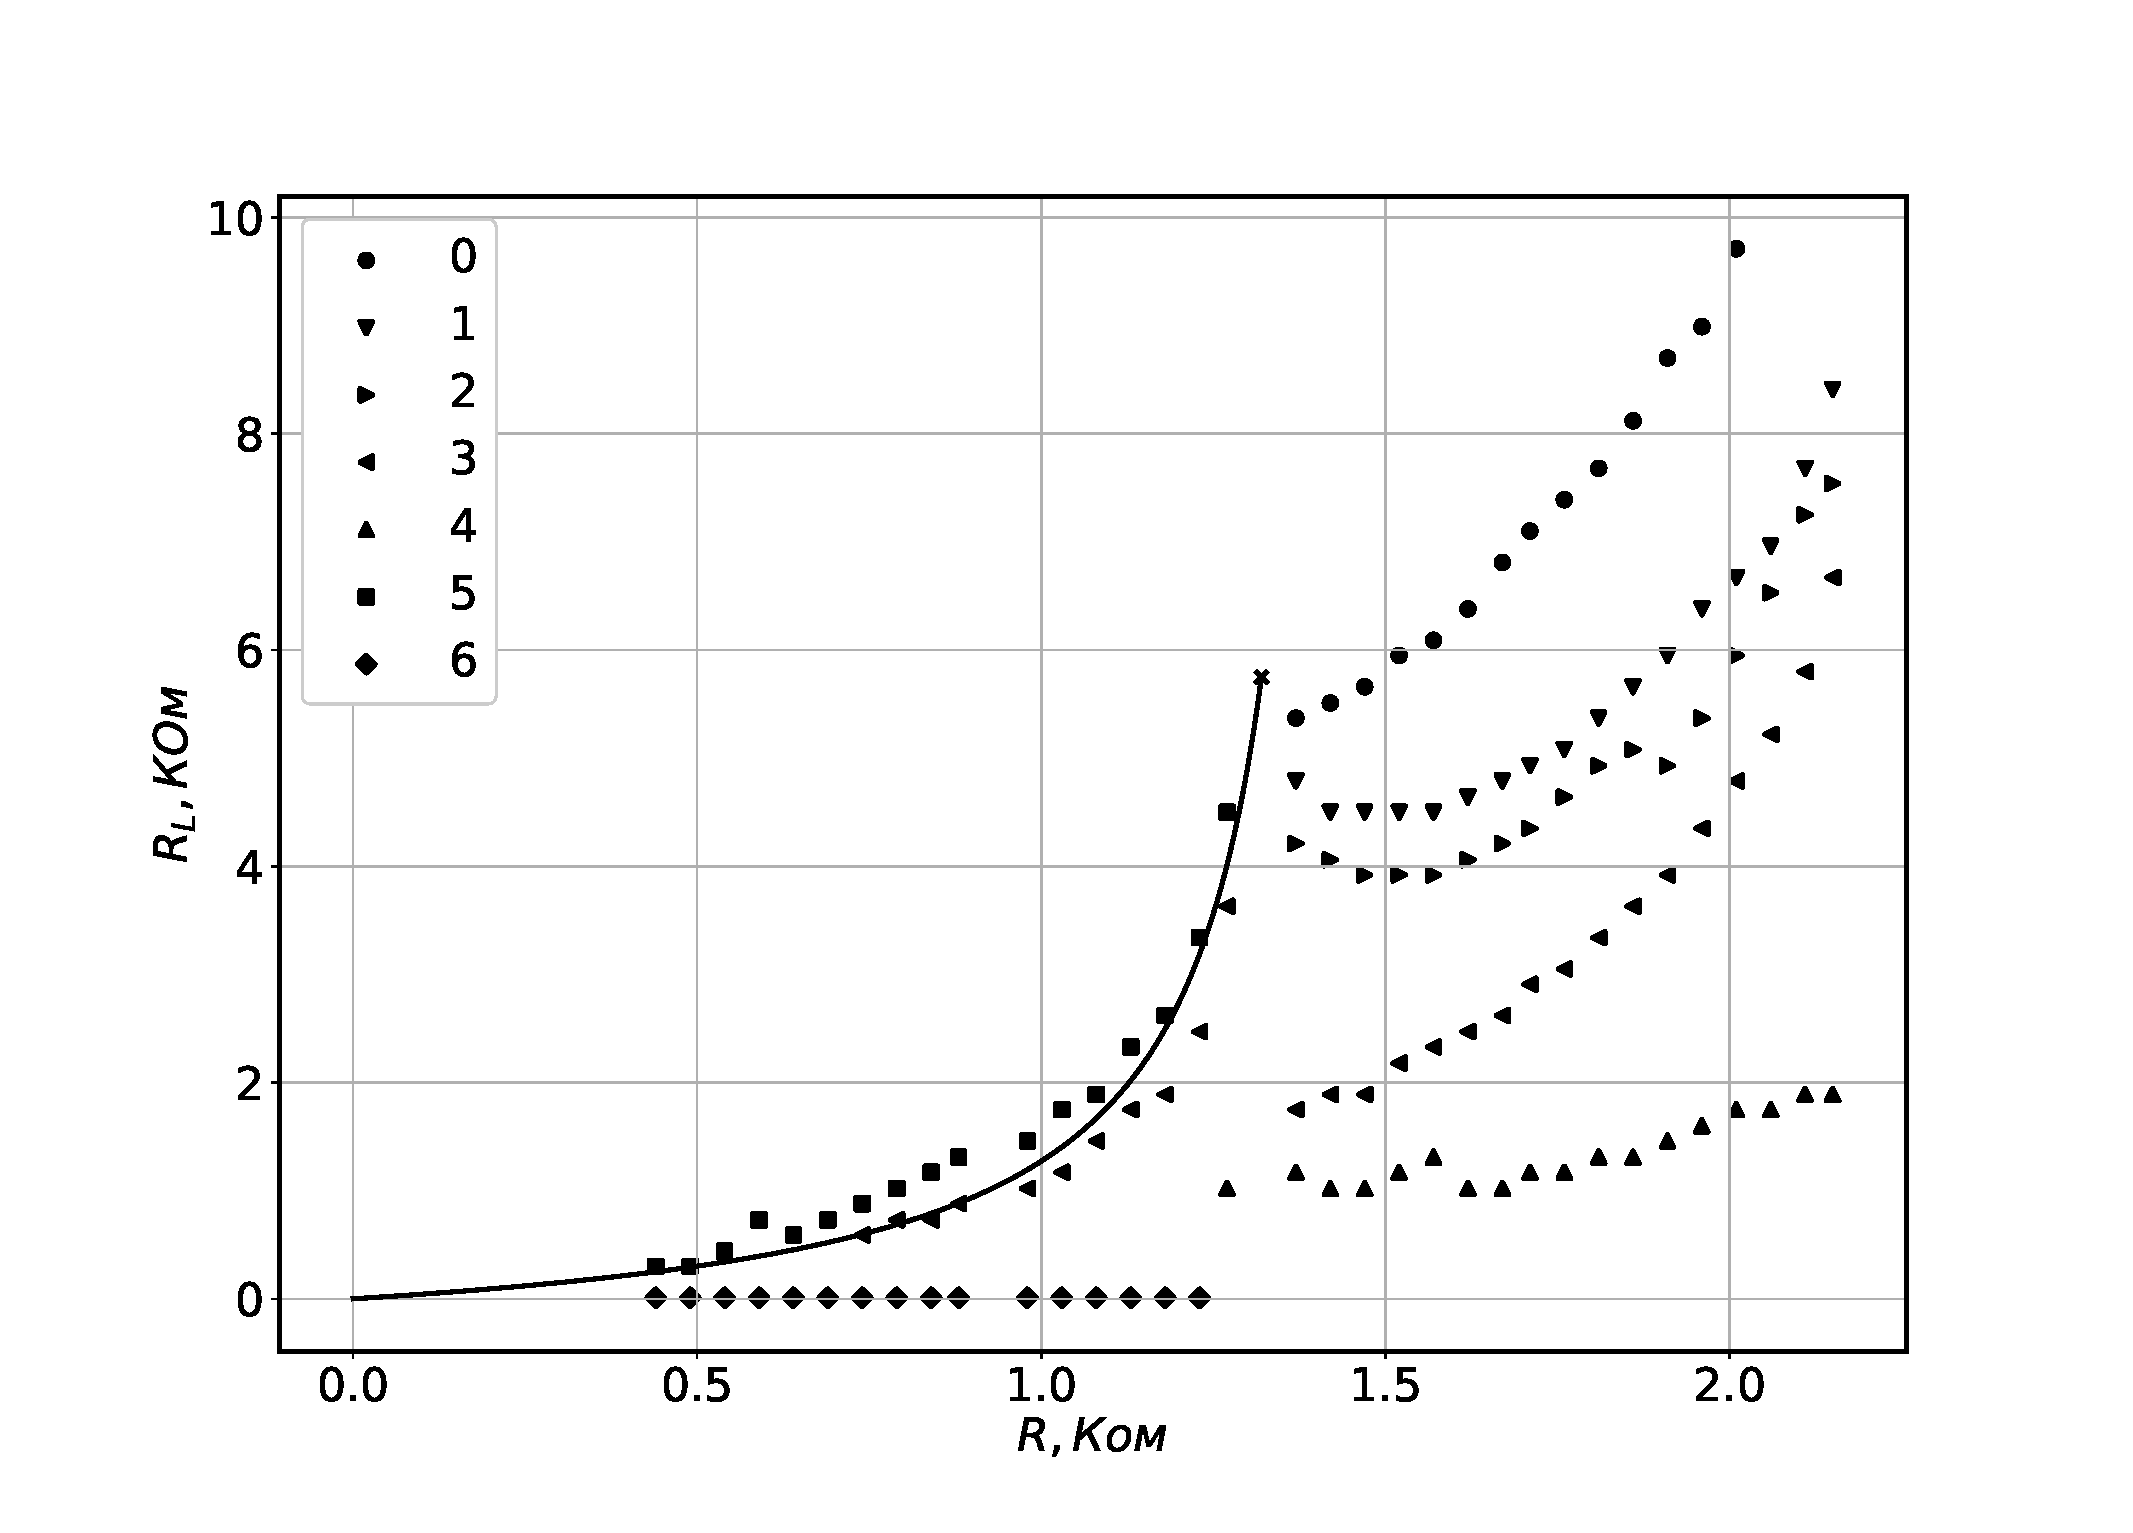
\includegraphics[width=0.75\textwidth]{critical_line_teor.eps}
	\caption{Бифуркационная диаграмма схемы Чуа, с нанесённой на неё критической кривой для устойчивости нулевого положения равновесия.}
	\label{fig:critical_line}
\end{figure}

\subsection*{Экспериментальная бифуркационная диаграмма системы}
Экспериментально была получена зависисмость состояния системы, возбуждаемое из положения равновесия. По 
полученным данным построена бифуркационная диаграмма (Рис. \ref{fig:real_bif_diag}). 
\begin{figure}[H]
	\centering
	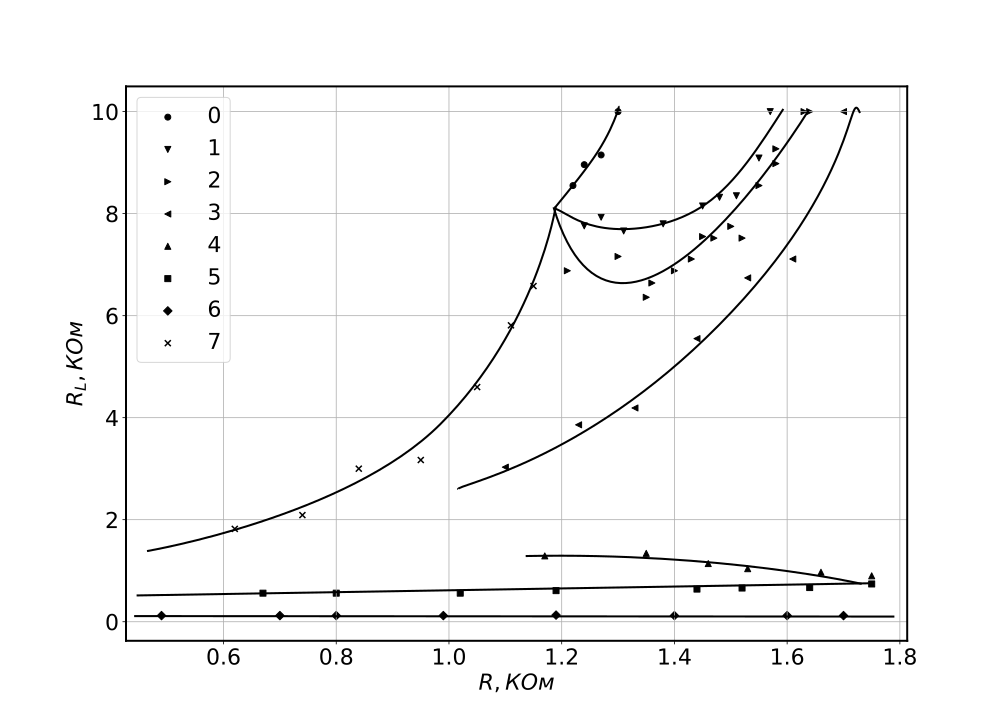
\includegraphics[width=0.75\textwidth]{bif_diag_lines.pdf}
	\caption{Реальная диаграмма состояний системы при различных $R$ и $R_L$. 
	Цифрами обозначены граничные кривые для состояний: 
	0 --- большой предельный цикл и двухпетлевой аттрактор,
	1 --- двухпетлевой аттрактор и аттрактор Рёсслера,\
	2 --- аттрактор Рёсслера и малый предельный цикл,
	3 --- малый предельный цикл и фокус, 
	4 --- фокус и малый предельный цикл, 
	5 --- малый предельный цикл и большой предельный цикл,
	6 --- большой предельный цикл и малый предельный цикл,
	7 --- большой предельный цикл и малый предельный цикл.}
	\label{fig:real_bif_diag}
\end{figure}
ТУТ ТОЖЕ НУЖНО ОПИСАТЬ ГРАФИК И СРАВНИТЬ С ПРЕДЫДУЩИМ. Также сюда прикрепить картинки и фото.


\subsection*{Нахождение параметров расхождения}
Так как хотя бифуркационные диаграммы в симуляции и в эксперименте и имеют схожий качественный вид, они 
расходятся в количественном смысле. Попытаемся найти какие параметры схемы отличаются от номинальных.
Легко определить, как изменилось сопростивление $G_a$, так как $R$ координата точки пересечения кривых 
равна $R = -\frac{1}{G_a}$, из чего получаем значение
\[
	G_e = (-8.3 \pm 0.8) \cdot 10^{-4} \text{ Ом}^{-1}, 
\]    
Что отличается от предполагаемой примерно на $10\%$, что укладывается в заявленную погрешность резисторов и 
не может создавать существенного изменения в поведении системы.  
Следующими элементами, для которых возможны отклонения от истинных значений являются конденсаторы. 
Для нахождения отклонения их параметров использована полученная теоретическая зависимость критической кривой устойчивости \ref{eq:R_crit}. 
Построена зависимость в линеаризованных координатах (Рис. \ref{fig:fit_coefs_line}): 
\[
	\frac{1}{R} \left( \frac{1}{R_L} \right) = -\frac{\alpha}{\alpha + 1} G_a - \frac{C_1}{(\alpha + 1) G_a k_L} \cdot \frac{1}{R_L},
\]
где $k_L = \frac{R_7 R_9 C}{R_8}$. 

\begin{figure}[H]
	\centering
	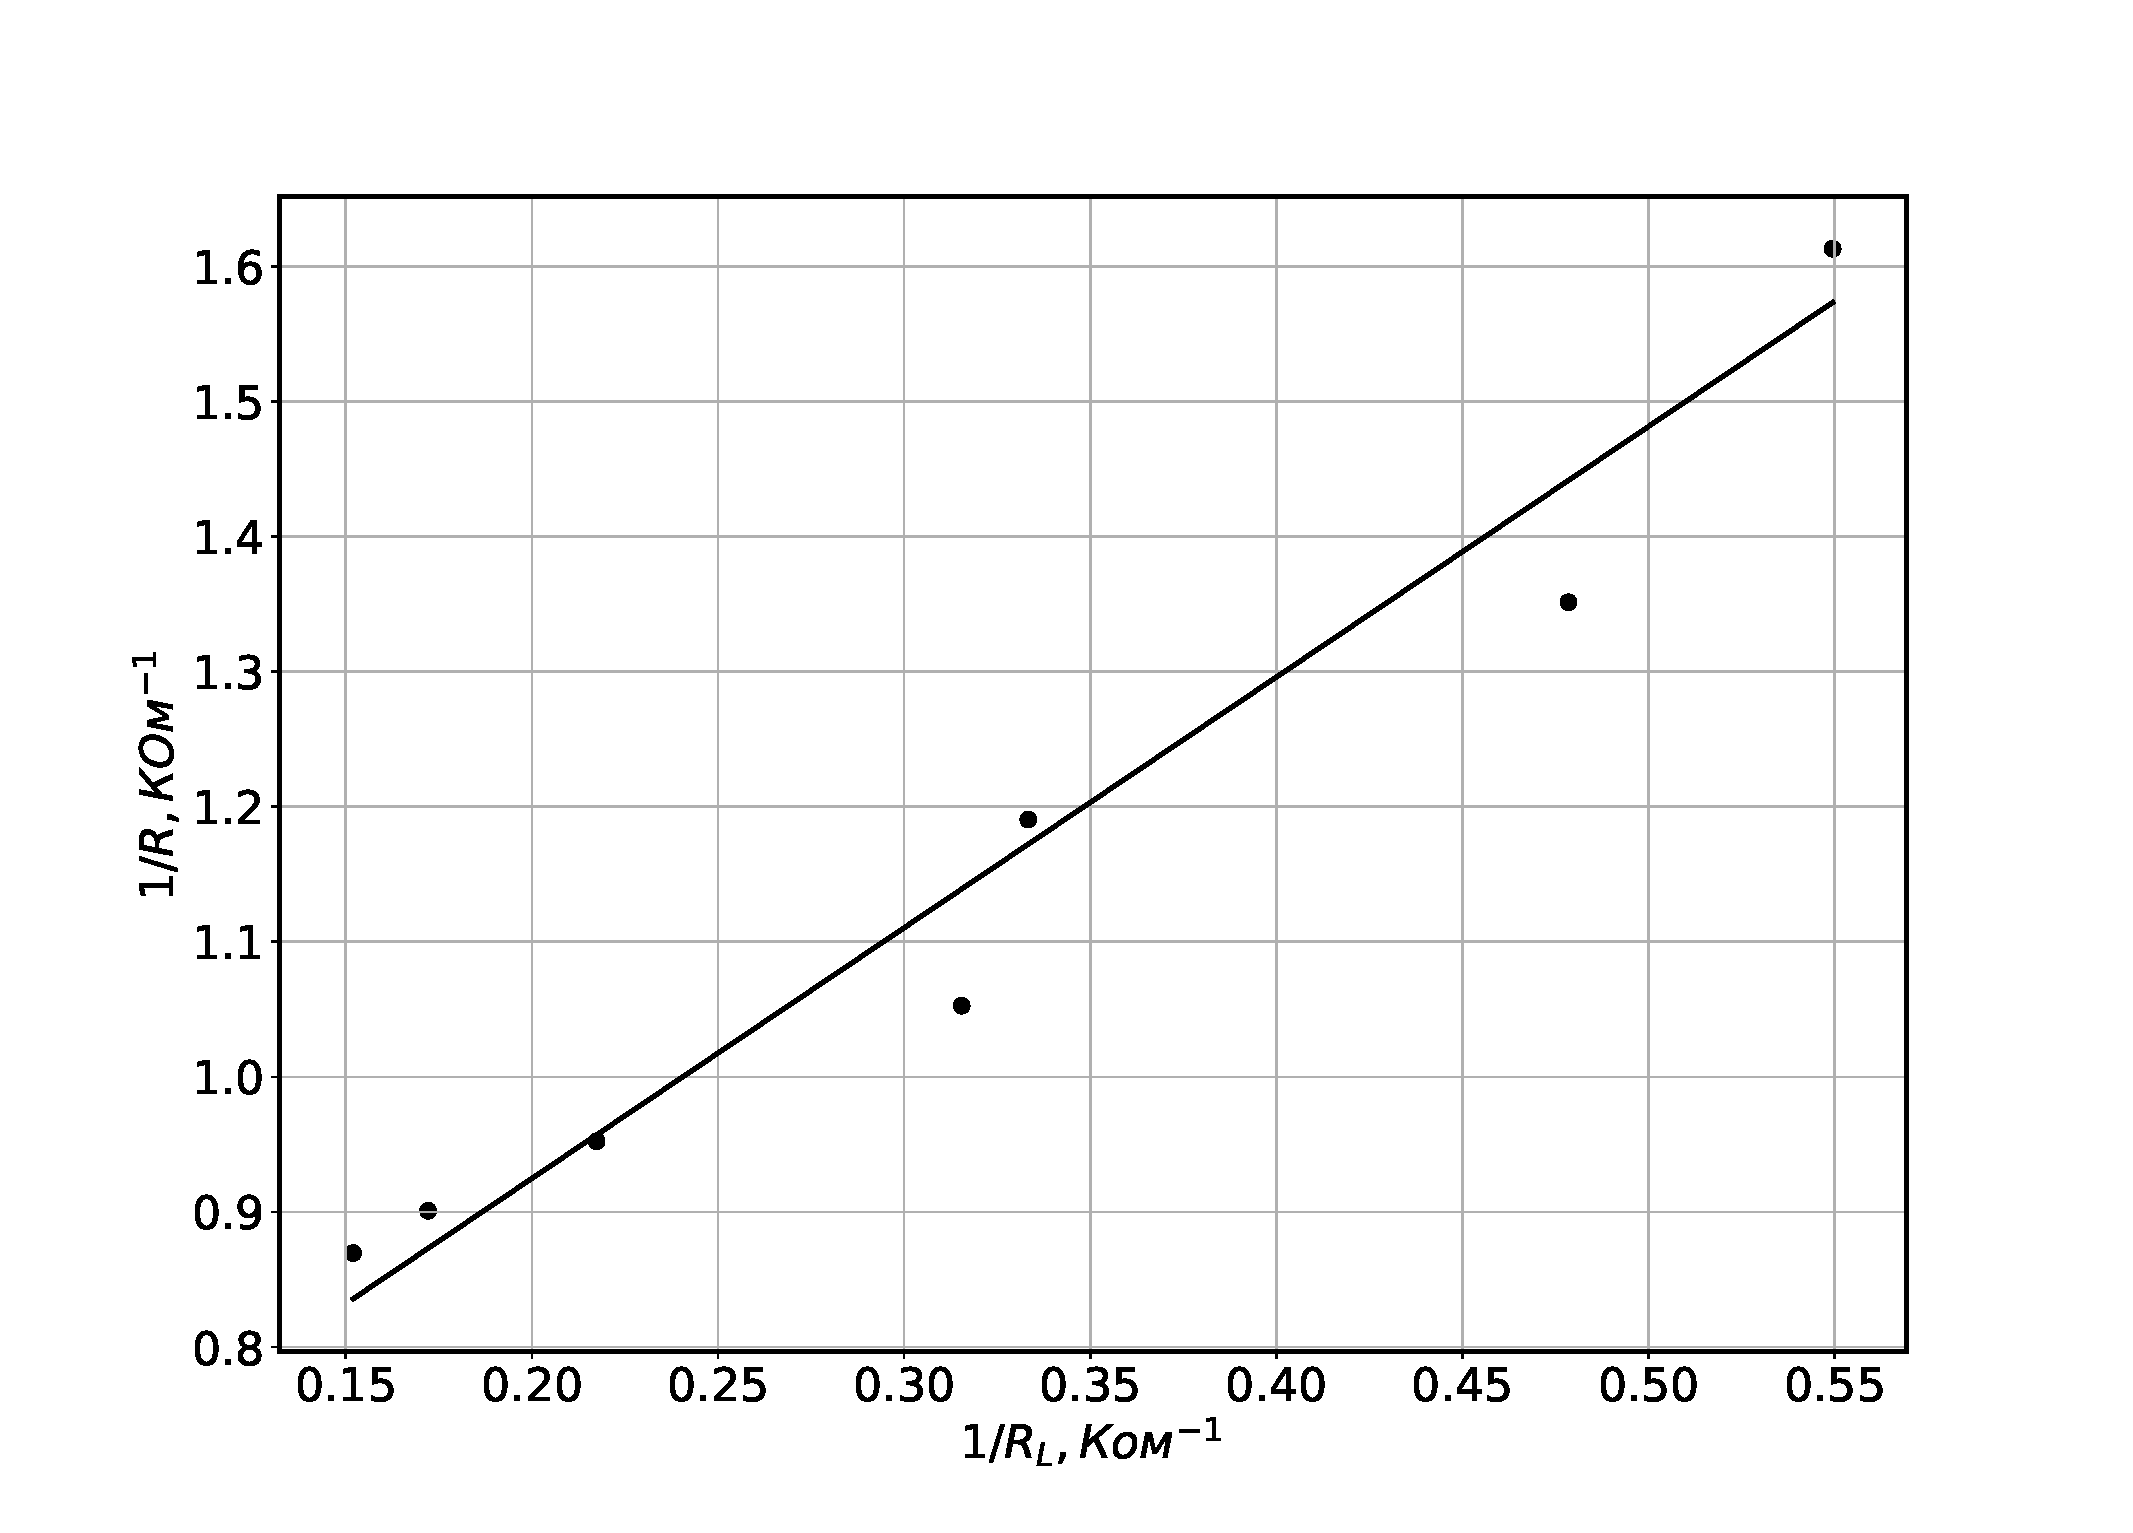
\includegraphics[width=0.75\textwidth]{fit_coefs_linear.eps}
	\caption{Линеаризованная зависимость критической кривой перехода $\frac{1}{R}$ от $\frac{1}{R}$ 
	между большим предельным циклом и малым предельным циклом.}
	\label{fig:fit_coefs_line}
\end{figure}

Полученные коэффициенты линейной зависимости составили: 
\[
	\begin{dcases}
		-\frac{\alpha}{\alpha + 1} G_a = 0.62 \pm 0.04 \text{ КОм}^{-1}, \\ 
		- \frac{C_1}{(\alpha + 1) G_a k_L} = 1.58 \pm 0.16.
	\end{dcases}
\]
Из первого коэффициента находим параметр $\alpha$, при этом используем экспериментальное значение $G_a$: 
\[
	\alpha = 2.9 \pm 0.2.
\]
Нахождение остальных параметров не может оказаться точным, так как коэффициент $k_L$ также зависит от ёмкости 
конденсатора и может изменяться. Однако в нашей оценке примем его неизменным и равным теоретическому, в таком случае 
можно найти $C_1$ и $C_2$: 
\[
	\begin{dcases}
		C_1 = 17 \pm 3 \text{ нФ}, \\
		C_2 = 53 \pm 6 \text { нФ}.
	\end{dcases}
\]    
Эти значения сильно отличаются от закладываемых в схему 
\[
	\begin{dcases}
		C_{1t} = 10 \text{ нФ}, \\
		C_{2t} = 100 \text{ нФ}.  
	\end{dcases}
\]
Такое поведение конденсаторов можно связать с эффектом понижения ёмкости керамических конденсаторов с повышением напряжения (Рис. \ref{fig:C_decrease}).
Таким образом, лучше использовать другие виды конденсаторов для построения схем Чуа, однако даже при таких отклонениях получается 
найти хаотические режимы схемы.

\begin{figure}[H]
	\centering
	\includegraphics[width=0.65\textwidth]{decrease_graph.png}
	\caption{График ёмкости керамических конденсаторов от напряжения \cite{Habr_C}.}
	\label{fig:C_decrease}
\end{figure}

\subsection*{Измерение амплитуды сигнала }
Для демонстарции динамики размера системы, при фиксированном $R$ была измерена зависимость 
амплитуды сигнала в зависимости от $R_L$ (Рис. \ref{fig:amplitudes_fix_R}).  

ПОСТРОИТЬ ГРАФИК И ОПИСАТЬ. 

\subsection*{Измерение размеров аттрактора Рёсслера}
Так как экспериментально было получено, что в отличие от симуляции, аттрактор 
Рёсслера занимает намного большую область на бифуркационной диаграмме, были измерены 
его размеры в зависимости от параметров $R$ и $R_L$. Получены трёхмерные графики зависимости угла поворота аттрактора и 
его поперечного размера от $R_L$ и $R$ (Рис. \ref{fig:Ressler_amplitudes}).

ПОСТРОИТЬ ГРАФИК И ОПИСАТЬ. 


\section*{Выводы}

\begin{thebibliography}{9}
	\bibitem{chuacircuits}
	https://www.chuacircuits.com
	\bibitem{Habr_C}
	Изменение ёмкости керамических конденсаторов от температуры и напряжения https://habr.com/ru/articles/384833/
\end{thebibliography}

\section*{Приложения}
\subsection*{Характеристики используемой схемы Чуа}
В качестве операционных усилителей были использованы TL082CP.
\begin{table}[H]
	\centering
	\begin{tabular}{|r|r|r|r|r|r|}
		\hline
		$R_1$ & $220$ Ом   & $R_6$  & $3.3$ КОм  & $R$   & $4.7$ КОм \\ \hline
		$R_2$ & $220$ Ом   & $R_7$  & $100$ Ом   & $C$   & $100$ нФ  \\ \hline
		$R_3$ & $2.2$ КОм  & $R_8$  & $3.3$ КОм  & $C_1$ & $10$ нФ   \\ \hline
		$R_4$ & $22.0$ КОм & $R_9$  & $1.0$ КОм  & $C_2$ & $100$ нФ  \\ \hline
		$R_5$ & $22.0$ КОм & $R_{10}$ & $10.0$ КОм &       &           \\ \hline
	\end{tabular}
	\caption{Характеристики используемых элементов.}
	\label{tab:curcuit_chars}
\end{table}
\end{document}